\chapter{Plataforma de trabajo} \label{chap:plataforma_trabajo}

Una vez establecidos los objetivos del proyecto y habiendo explorado el contexto de la inteligencia artificial en la industria del videojuego, es fundamental detallar la plataforma sobre la cual se ha erigido el trabajo práctico. Este capítulo se dedica a describir en profundidad los dos pilares que constituyen el campo de pruebas del agente: el videojuego de cartas \textit{Tales of Tribute} y, de forma más importante, su \textbf{motor de simulación de código abierto}, \textit{Scripts of Tribute}. Para poder comprender las decisiones que se han tomado durante el desarrollo del bot, es necesario conocer primero las reglas del entorno en el que opera. Por ello, se comenzará explicando las reglas y mecánicas del videojuego. Posteriormente, se analizará la arquitectura del entorno de simulación, que no solo hace posible el enfrentamiento entre bots, sino que también ha servido de base para competiciones académicas internacionales.


\section{El videojuego: \textit{Tales of Tribute}} \label{sec:tales_of_tribute}

\textit{Tales of Tribute} es un videojuego de cartas para dos jugadores del género de construcción de mazos, que existe dentro del popular videojuego \textit{The Elder Scrolls Online}. En la figura \ref{fig:tales_tablero} se puede ver una captura del tablero de juego, donde se han numerado los elementos principales para facilitar su identificación \cite{pixel_eso_2022}.

El objetivo principal del juego es conseguir puntos de prestigio\footnote{El prestigio es la métrica principal de victoria en \textit{Tales of Tribute}. Se podría considerar un análogo a los ``puntos de vida'' en otros juegos, pero en este caso, el objetivo es acumularlos en vez de reducir los del oponente.}, el cual se puede consultar en su marcador (elemento 11 en la figura \ref{fig:tales_tablero}). Hay varias formas de ganar: un jugador consigue la victoria si alcanza 40 puntos de prestigio y mantiene la ventaja tras el turno de su oponente. Si no lo consigue, el juego continúa hasta que alguno de los dos jugadores alcance los 80 puntos. Existe, además, una condición de victoria alternativa que se consigue al ganarse el favor de todos los ``patrones'', un tipo de mecánica especial que se detallará más adelante.

\begin{figure}[H]
	\centering
	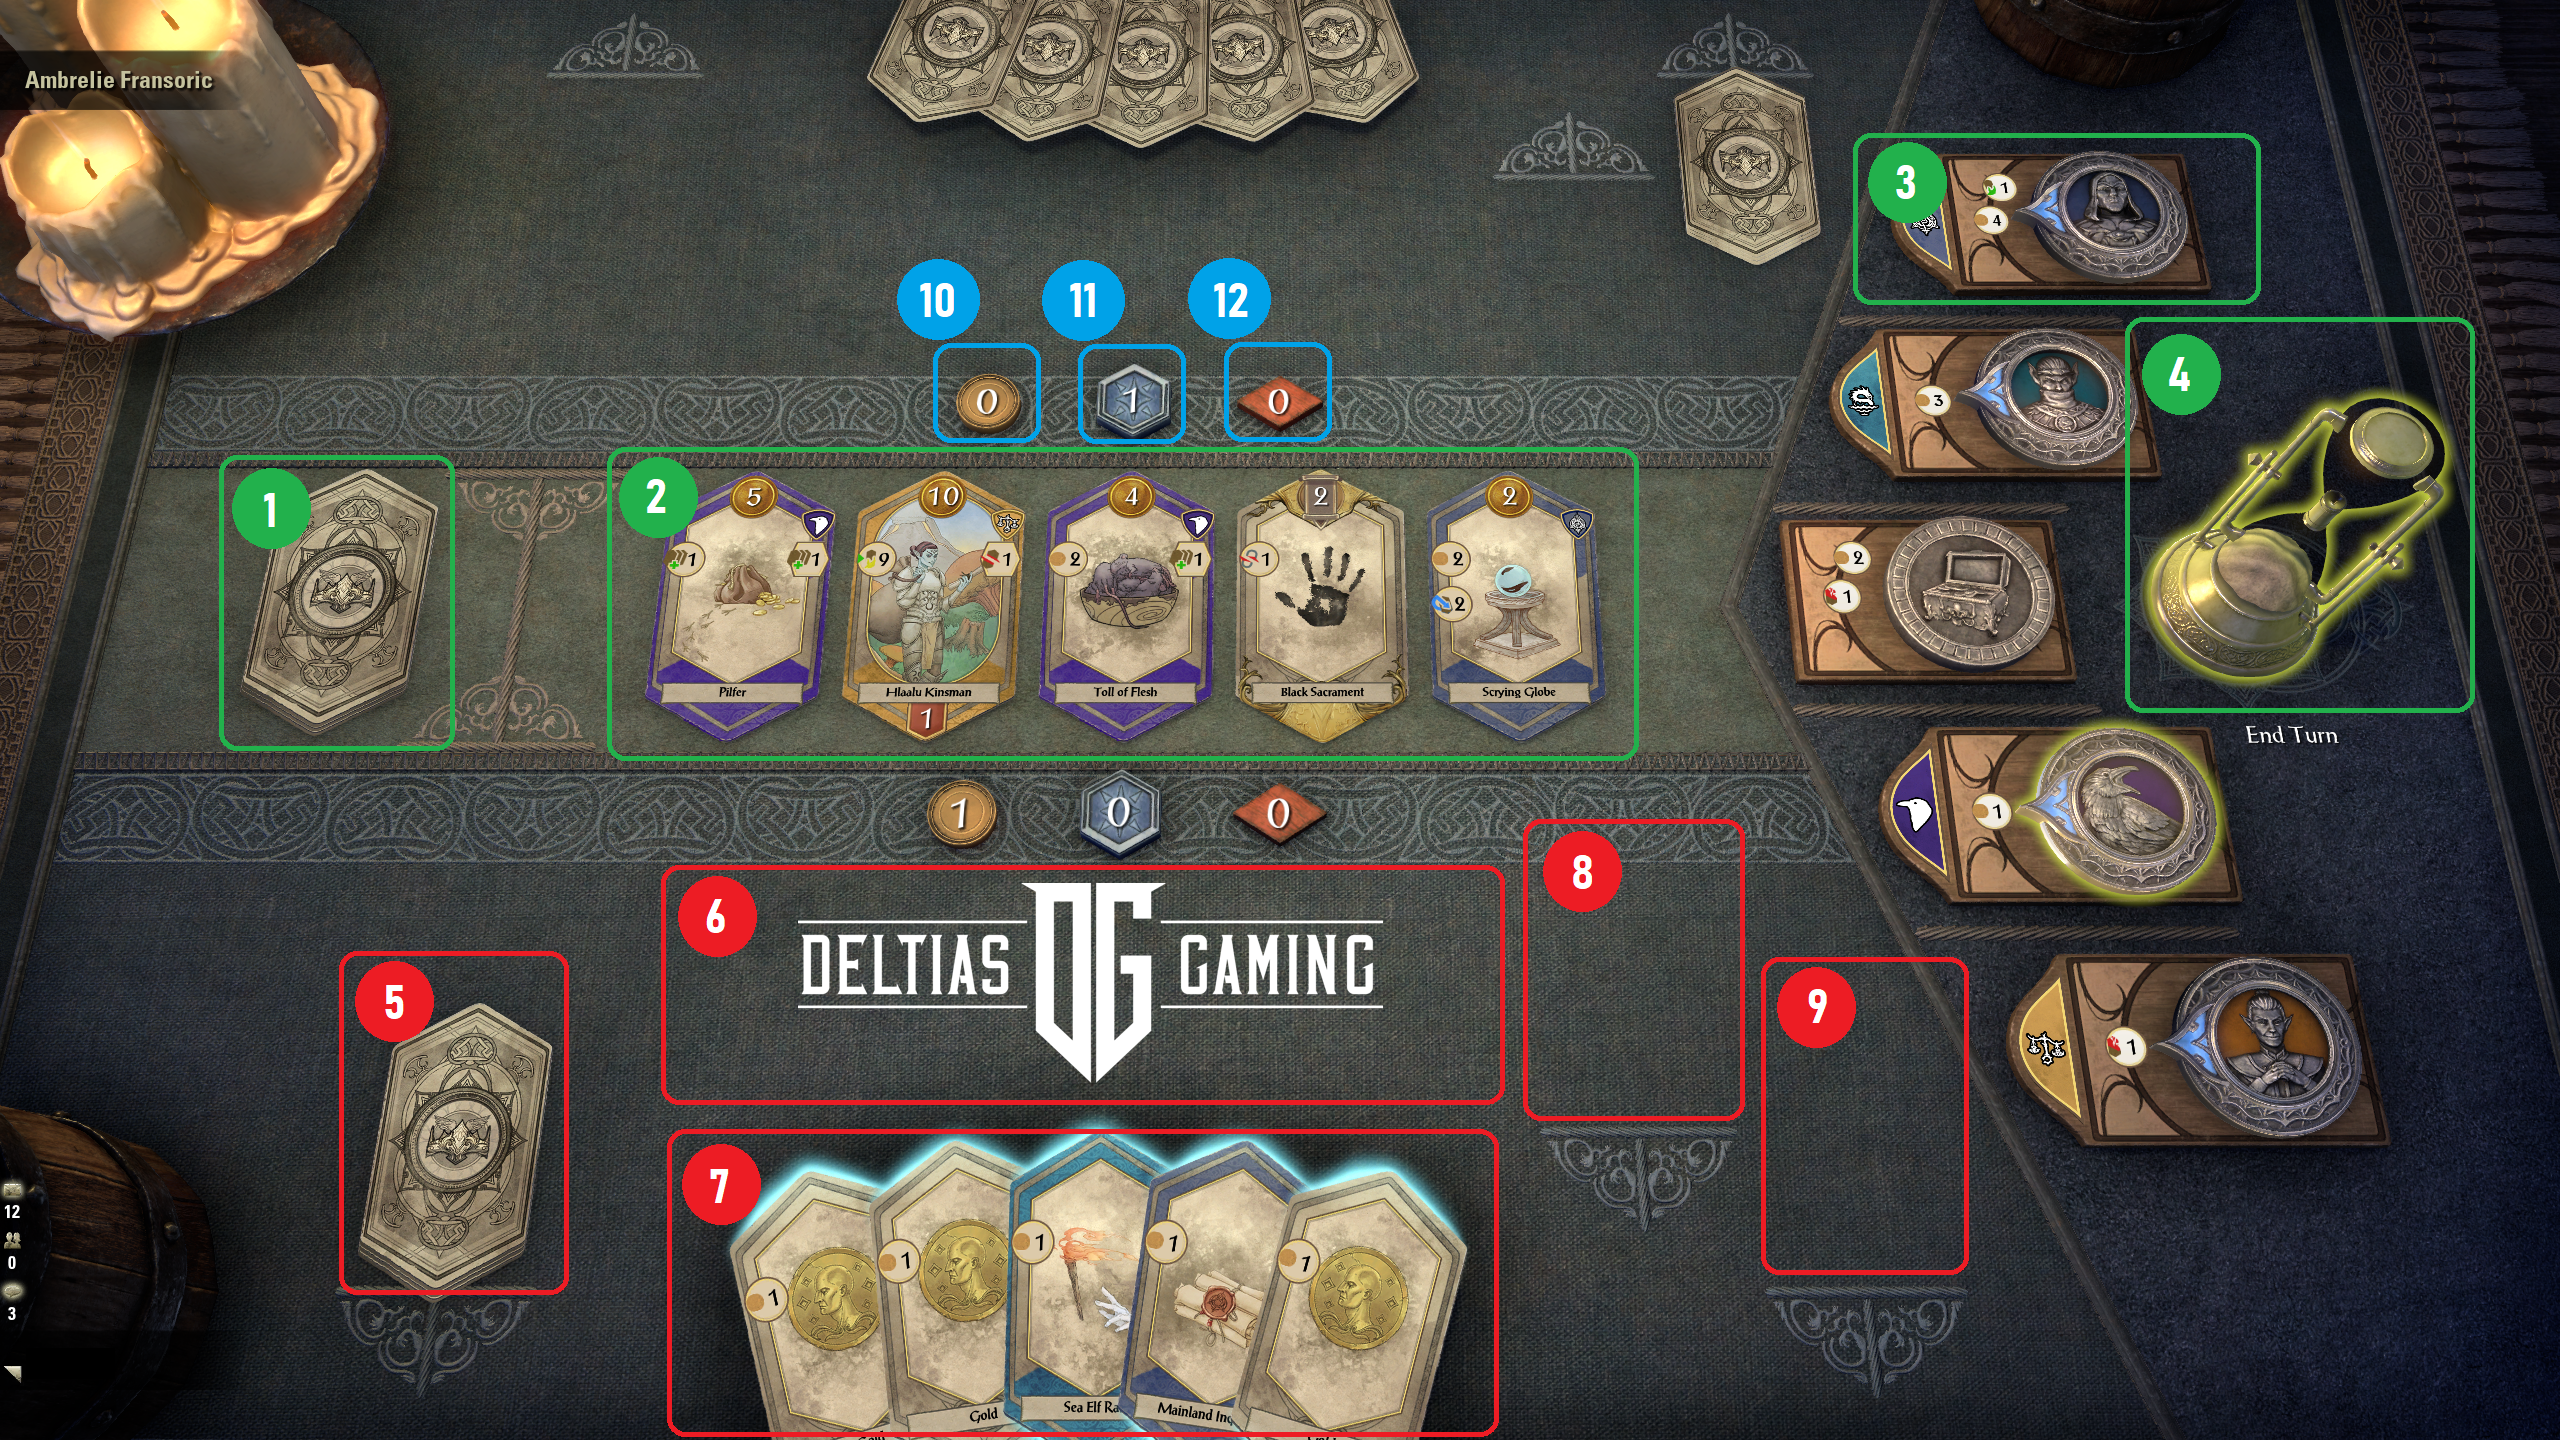
\includegraphics[width=1.0\textwidth]{img/tales_tablero.png}
	\caption{Tablero de juego de Tales of Tribute, con sus componentes principales numerados. \cite{pixel_eso_2022}}
	\label{fig:tales_tablero}
\end{figure}

Al comienzo de cada partida, ambos jugadores deben elegir con qué conjuntos de cartas quieren jugar. Para ello, se presentan siete mazos, cada uno asociado a un patrón (elemento 3), y los jugadores se turnan para seleccionar un total de cuatro. Estos cuatro mazos, junto con un mazo estándar asociado a la ``Tesorería'' que está presente en todas las partidas, se barajan conjuntamente para formar el mazo de robo de la Taberna (elemento 1). De este mazo se revelan cinco cartas en el área de la Taberna (elemento 2), que son las cartas que los jugadores podrán adquirir durante la partida. La esencia de la construcción de mazos reside en que ambos jugadores comienzan con un pequeño mazo de diez cartas básicas idénticas y, a lo largo de la partida, utilizan los recursos que estas generan para comprar cartas más poderosas de la Taberna, añadiéndolas a su propio ciclo de cartas. Además, el jugador que tiene el turno en segundo lugar obtiene una pequeña recompensa de 1 moneda debido a que cuenta con la desventaja de que su oponente ha podido jugar primero.

La estructura de un turno es la siguiente, el jugador activo roba cinco cartas de su mazo personal (elemento 5) para formar su mano (elemento 7). Jugar una carta no tiene coste y, al hacerlo, se activan sus efectos y se mueve a una pila de descarte temporal (elemento 8). Al final del turno, todas las cartas sin jugar aun en la mano y en la pila de descarte temporal se mueven a la pila de reposo (elemento 9). Cuando el mazo de robo personal se agota, la pila de reposo se baraja y se convierte en el nuevo mazo de robo, completando el ciclo. De esta manera, las cartas adquiridas se incorporan progresivamente al mazo del jugador, haciéndolo cada vez más potente.

Las cartas se pueden clasificar en dos tipos principales: acciones y agentes. Las ``cartas de acción'' producen un efecto inmediato (como ganar monedas u obtener puntos de poder) y después se descartan. Por otro lado, las ``cartas de agente'' también tienen un efecto inmediato, pero tras jugarse, se colocan en el tablero en la zona de agentes activos (elemento 6). Estos agentes permanecen en juego y su habilidad puede ser activada una vez por turno, proporcionando una ventaja continua. Sin embargo, el oponente puede destruirlos de diferentes maneras, como utilizando puntos de poder (elemento 12), donde cada punto inflige un punto de daño al agente. Existen, además, las ``cartas de contrato'', que son versiones de un solo uso de las acciones y agentes, siendo eliminadas del juego permanentemente tras su primer uso o al ser derrotadas. Este tipo de cartas de contrato son las que se han utilizado para crear heurísticas específicas en el bot, ya que sus efectos pueden ser muy poderosos.

Finalmente, además de jugar y comprar cartas, los jugadores disponen de otras acciones estratégicas. La más importante es la posibilidad de interactuar con uno de los cuatro patrones elegidos al principio de la partida. Cada patrón ofrece una habilidad única a cambio de un coste en monedas, poder u otros activos. Su estado puede cambiar de neutral a favorable o desfavorable según que jugador los active y la perspectiva desde donde se mire. Ganarse el favor de todos los patrones es, como se mencionó, una de las condiciones de victoria. Por último, una mecánica muy importante es que muchas cartas poseen efectos de ``combo'', lo cuales se activan si en el mismo turno se han jugado previamente otras cartas del mismo mazo o patrón, incentivando así la creación de mazos con sinergias.

\section{El entorno de simulación: \textit{Scripts of Tribute}} \label{sec:scripts_of_tribute}

Para poder entrenar y evaluar un agente de inteligencia artificial de forma automática, es imprescindible contar con un entorno que permita la simulación de partidas paralelamente y sin intervención humana. Para cumplir esa función, se utilizó \textit{Scripts of Tribute}, que es un motor de simulación de partidas de código abierto que reimplementa las reglas de una versión específica\footnote{La versión en concreto ha ido avanzando con el desarrollo del motor.} de \textit{Tales of Tribute}. Desarrollado en C\# sobre el framework .NET 8, su propósito principal es servir como un banco de pruebas para la investigación y competición de IA, permitiendo la creación de agentes autónomos y así como su enfrentamiento. El motor se divide en dos componentes principales: un cliente con interfaz gráfica para la visualización y depuración, y una aplicación de consola para la ejecución masiva de simulaciones, siendo este último el componente esencial para el entrenamiento evolutivo.

\subsection{Interfaz gráfica} \label{sec:gui_scripts_of_tribute}

Aunque el entrenamiento de este proyecto se basa en la ejecución de simulaciones desde la consola de comandos, el ecosistema de SoT cuenta con un cliente gráfico desarrollado en el motor Unity. Esta herramienta permite visualizar las partidas en tiempo real, tanto entre bots como entre jugador humano y bot. Como se puede observar en la figura \ref{fig:game_view}, la interfaz replica el tablero de juego de \textit{Tales of Tribute}.

\begin{figure}[H]
	\centering
	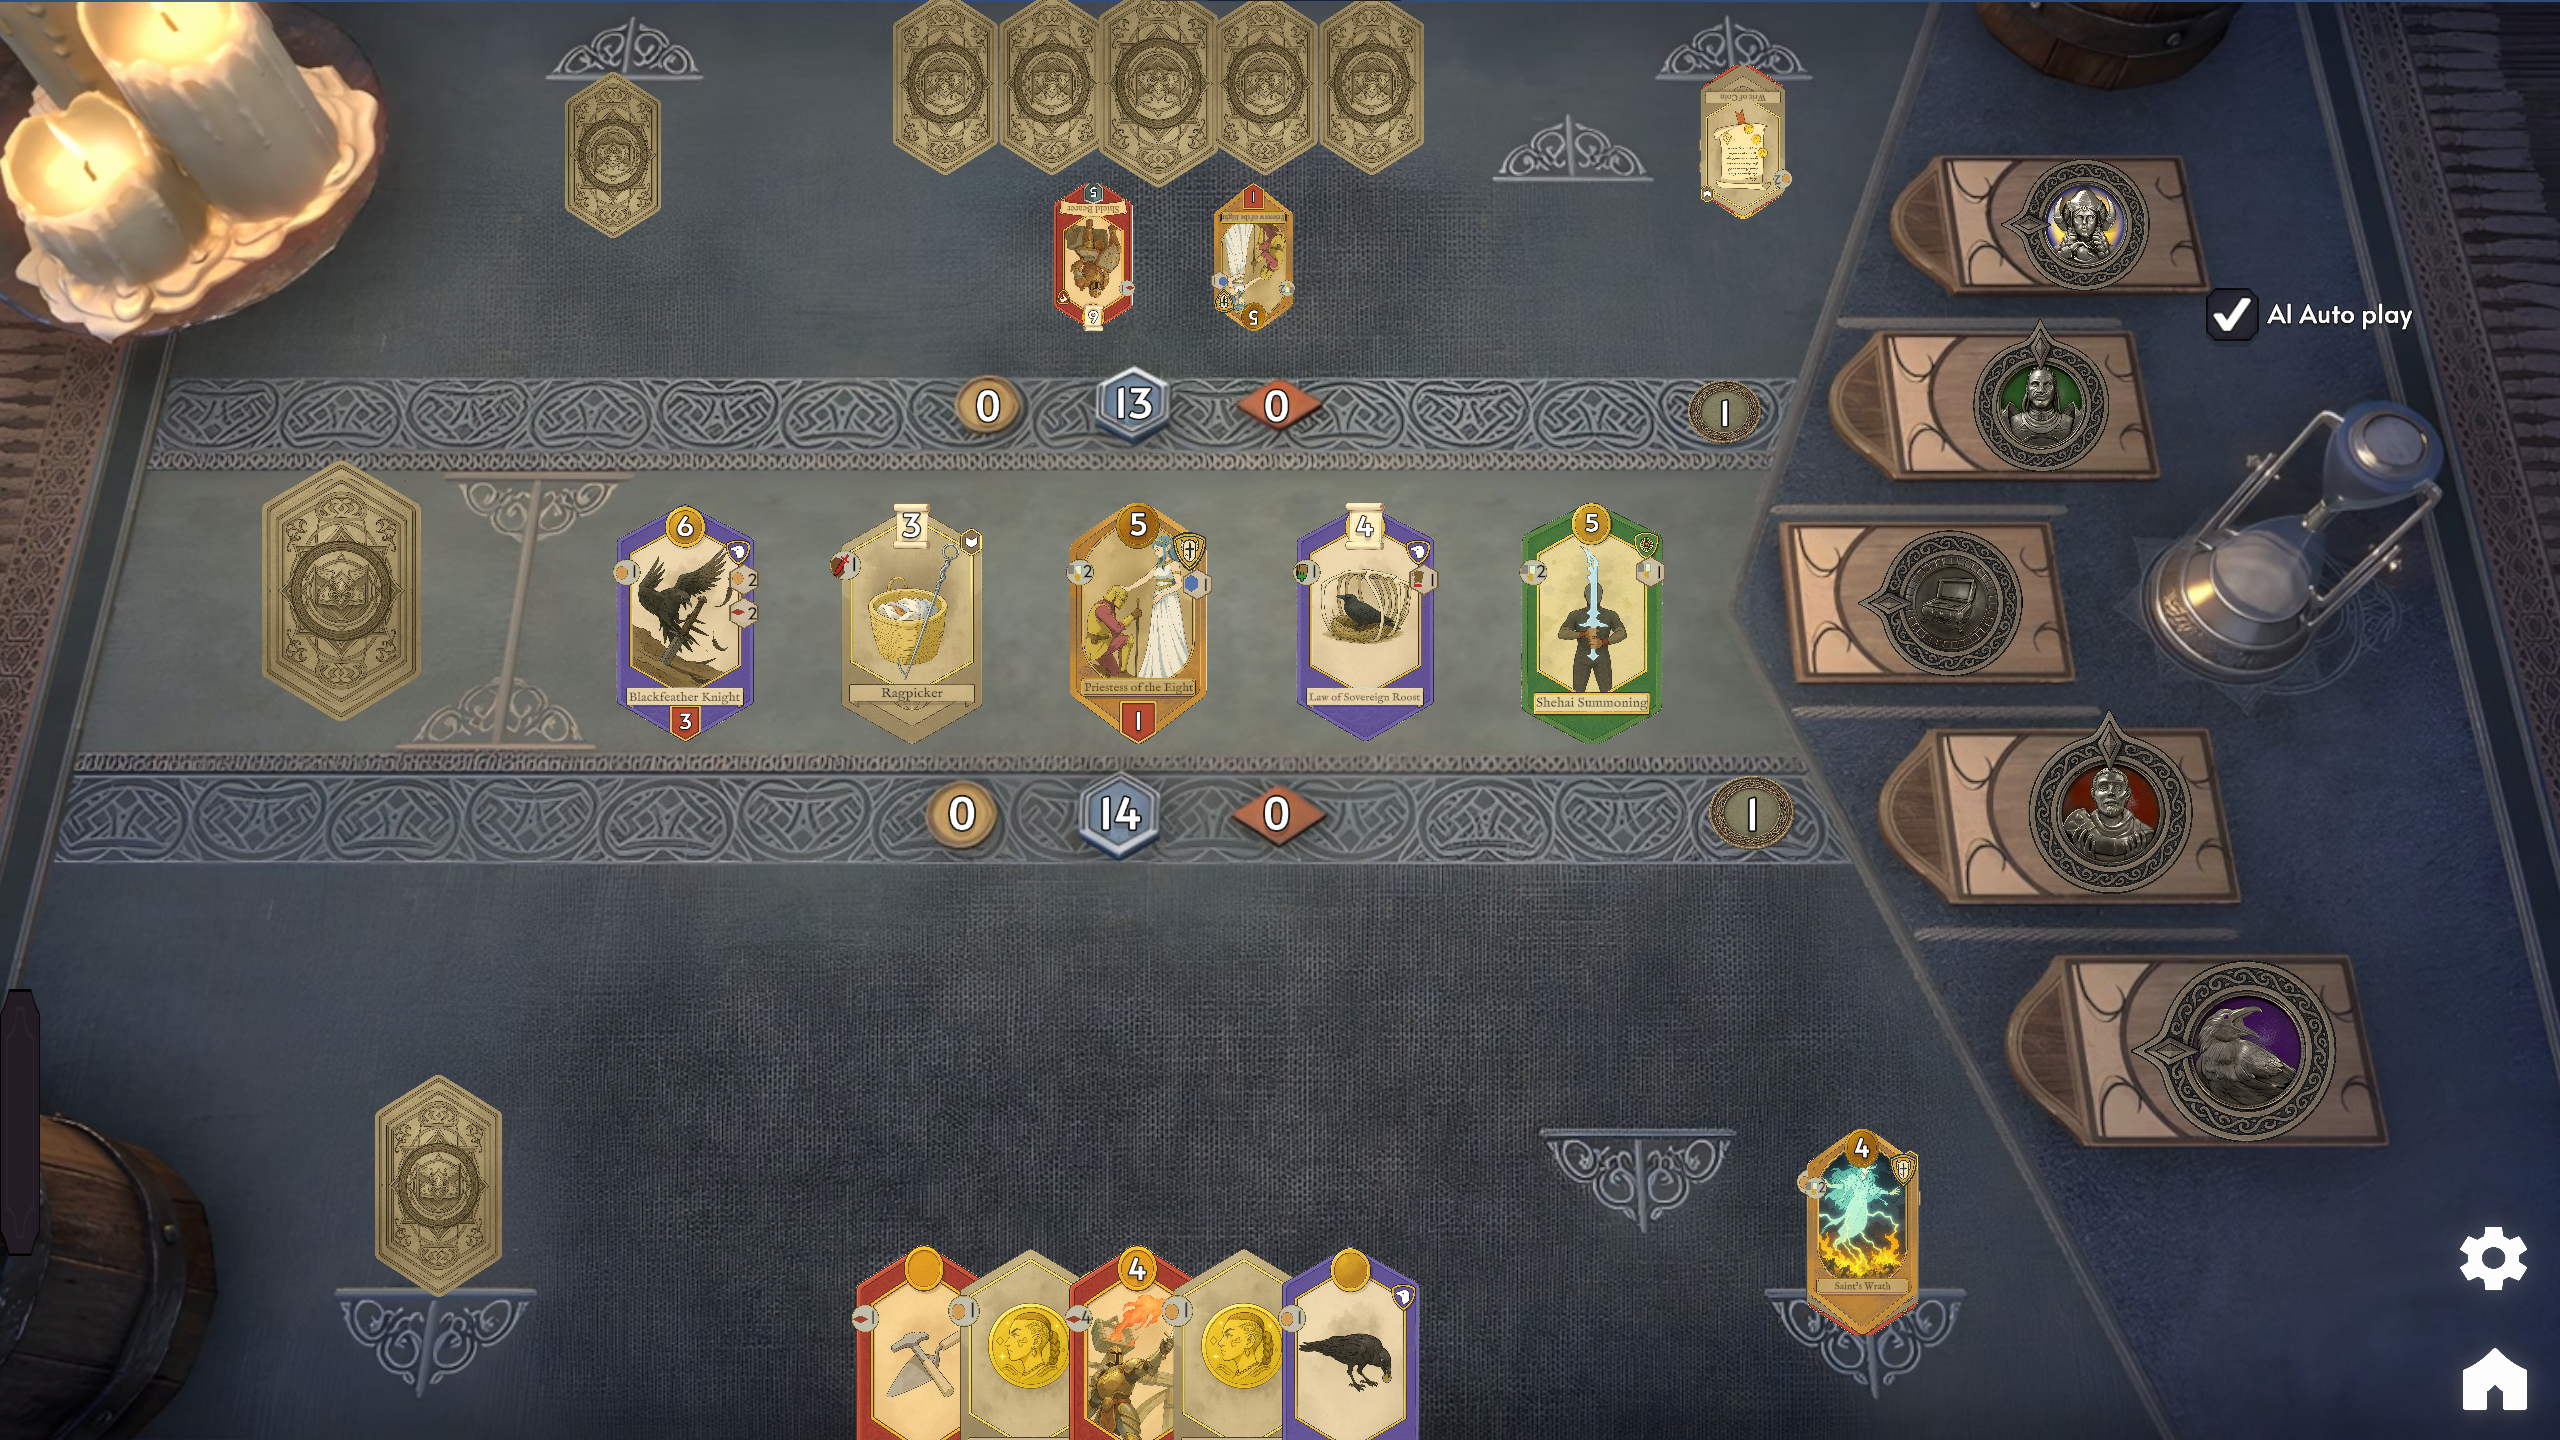
\includegraphics[width=1.0\textwidth]{img/GameView.png}
	\caption{Tablero de juego de SoT. \cite{ematerasu_scriptsoftribute-gui-20_2025}}
	\label{fig:game_view}
\end{figure}

El cliente gráfico también cuenta con pantallas específicas para las acciones especiales, en la figura \ref{fig:choice_panel} se muestra un ejemplo del panel de elección de descarte de cartas.

\begin{figure}[H]
	\centering
	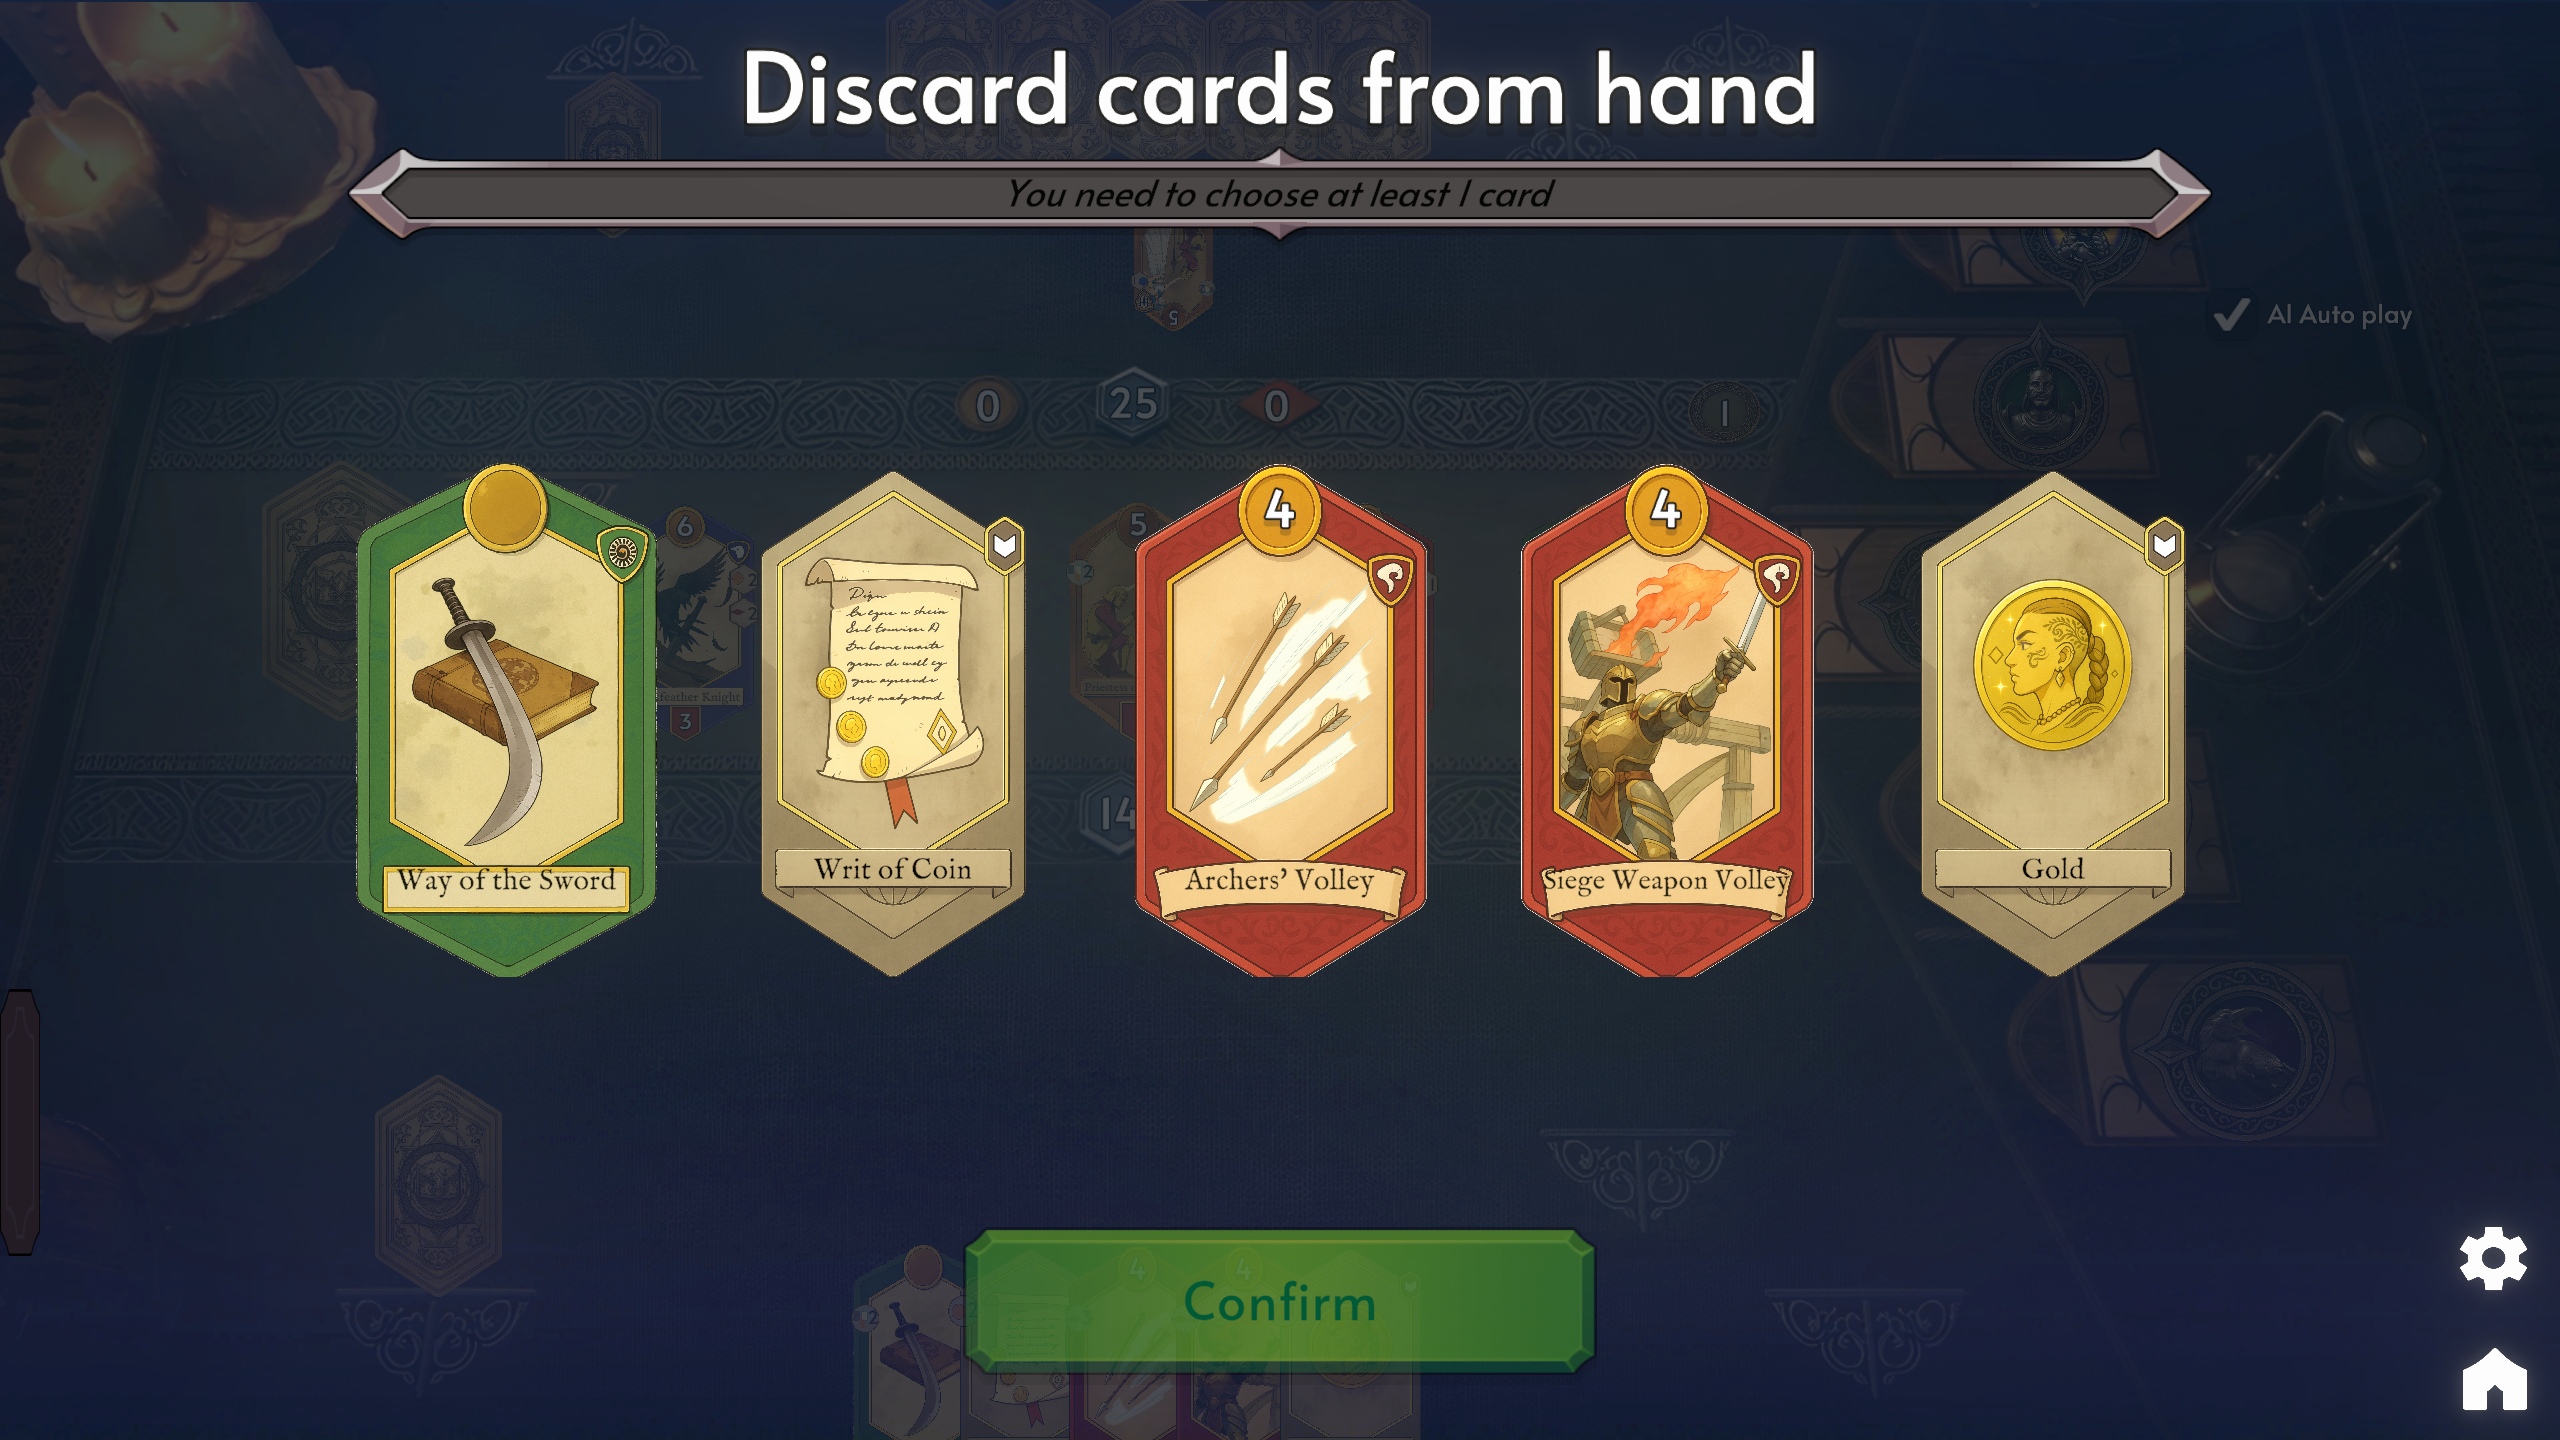
\includegraphics[width=1.0\textwidth]{img/ChoicePanel.png}
	\caption{Vista de elección de cartas en SoT. \cite{ematerasu_scriptsoftribute-gui-20_2025}}
	\label{fig:choice_panel}
\end{figure}

Finalmente, al concluir una partida, la interfaz presenta una pantalla de resumen como la de la figura \ref{fig:game_end}, donde se muestra el ganador y un historial completo de los movimientos realizados por ambos jugadores. Esto también se puede realizar con la versión de consola, pero la interfaz gráfica ofrece una visualización más intuitiva y accesible para el usuario.

\begin{figure}[H]
	\centering
	\includegraphics[width=1.0\textwidth]{img/GameEnd.png}
	\caption{Vista de final de partida con historial de movimientos en SoT. \cite{ematerasu_scriptsoftribute-gui-20_2025}}
	\label{fig:game_end}
\end{figure}

\subsection{Arquitectura del entorno} \label{sec:arquitectura_entorno}

El núcleo del motor de simulación, \textit{Scripts of Tribute-Core}, proporciona toda la lógica del juego y los puntos de entrada para el desarrollo de agentes. Para crear un nuevo bot, es necesario desarrollar una clase que herede de la clase abstracta ``AI.cs'' e implementar, como mínimo, dos métodos esenciales: ``SelectPatron'', que se encarga de la selección de patrones al inicio de la partida, y ``Play'', que se invoca repetidamente durante el turno del agente para que elija la siguiente acción a realizar. En cada llamada, el método ``Play'' recibe un objeto ``GameState'' que contiene una representación completa de toda la información visible en el juego, como las cartas en la mano, los agentes en el tablero o las cartas disponibles en la Taberna, permitiendo al bot tomar una decisión informada.

Si bien la interfaz gráfica es útil para la observación, la gran mayoría del trabajo de este proyecto se apoya en el ``GameRunner'', una aplicación de consola que forma parte del núcleo de SoT. Esta herramienta permite ejecutar un gran número de partidas entre dos bots especificados por línea de comandos, utilizando varios núcleos de la CPU para ejecutar tantas partidas simultáneas como se indique. Es precisamente este programa el invocado por el script de entrenamiento para cada una de las miles de evaluaciones que componen el proceso evolutivo.

Actualizaciones recientes en el motor han añadido la posibilidad de interactuar con agentes escritos en lenguajes externos mediante gRPC\footnote{gRPC es un sistema de código abierto desarrollado por Google para gestionar llamadas a procedimientos remotos (RPC) de alto rendimiento. Permite que un programa ejecute una función en otro proceso, incluso en una máquina diferente, como si fuera una llamada local \cite{google_grpc_2016}.}. Sin embargo, este proyecto inició su desarrollo antes de que esta funcionalidad estuviera disponible, por lo que el bot se tuvo que implementar en C\# y no en Python. Esto generó un problema de comunicación entre el script de entrenamiento y el bot, ya que el motor no permite la inyección de los pesos del bot directamente desde la línea de comandos. Para resolverlo, el script de ajuste de pesos (o ``entrenador'') establece los pesos del bot mediante variables de entorno del intérprete de comandos utilizado (ya sea bash o Powershell), que se leen a través de un método del bot antes de que comience la simulación. Esta dinámica permite que el algoritmo evolutivo en Python asigne pesos y evalúe el comportamiento del agente que opera dentro del entorno C\#.

Durante el continuo desarrollo del motor, Ematerasu et al. no solo han añadido nuevas opciones técnicas, sino también el nuevo contenido del juego. La edición de 2024 introdujo el mazo del patrón ``Rey Hechicero Orgnum'', mientras que la de 2025 añadió el de ``Santa Alessia''.

\section{La competición IEEE-CoG} \label{sec:competicion_ieee_cog}

Más allá de ser un simple motor de simulación, \textit{Scripts of Tribute} también se utiliza como plataforma para unas de las varias competiciones de inteligencia artificial celebradas anualmente en el congreso del \textit{IEEE Conference on Games} (CoG). El formato de la competición está diseñado para medir de forma robusta el rendimiento de los bots. Los agentes se enfrentan en un torneo de tipo \textit{Round-robin} (todos contra todos), donde el ganador se determina por el mayor porcentaje de victorias promedio tras un gran número de partidas espejo\footnote{En una ``partida espejo'', dos agentes A y B juegan una contra el otro dos veces, intercambiando la posición de jugador inicial en cada partida para asegurar la equidad.}. Las reglas imponen restricciones técnicas estrictas para los participantes, como un límite de tiempo de 10 segundos por turno y un uso de memoria que no debe exceder los 256 MB. Estas limitaciones obligan a los desarrolladores a buscar soluciones eficientes que equilibren la complejidad estratégica con el rendimiento computacional.

En la figura \ref{fig:competicion_ieee_cog_2024}, se muestran los resultados de la edición de 2024, donde el bot ya mencionado en la sección \ref{sec:mcts_cog} del capítulo anterior, gano por segundo a vez consecutiva. Los otros bots contaban con gran variedad de técnicas para su entrenamiento, desde MCTS hasta redes neuronales profundas e incluso aprendizaje por refuerzo.

\begin{figure}[H]
	\centering
	\includegraphics[width=1.0\textwidth]{img/ieee-cog-2024.png}
	\caption{Resultados de la competición IEEE-CoG 2024. \cite{ematerasu_scriptsoftribute-competitionsarchive_2024}}
	\label{fig:competicion_ieee_cog_2024}
\end{figure}

Este capítulo marca la conclusión del objetivo \textbf{OG1}, que consistía en analizar en profundidad las mecánicas del juego \textit{Tales of Tribute}, el entorno de desarrollo \textit{Scripts of Tribute} y adquirir las competencias necesarias en el lenguaje de programación C\#.